\chapter{水下图像合成研究}
海洋包含着未知的生物和巨大能源,对地球上生命延续起着重要的作用。自二十世纪中叶以来,高科技海洋勘测一直备受瞩目,视觉技术因能传达高密度信息而被应用在海洋环境中。研究人员致力于为水下机器人、水下救援、生态检测、海洋生物跟踪和实时导航等各种水下应用捕获高质量的水下图像。水下图像合成为水下应用的图像缺乏问题提供了一种行之有效的解决方式。

\section{水下图像成像原理及存在问题}
水下环境的特殊物理和化学特性严重影响了水下图像的质量和数量,产生许多比在地面成像的更难克服的问题。如图~\ref{fig:underwater}所示,水下成像存在的问题可以进行详尽分析。

\begin{figure*}[ht]
    \centering
	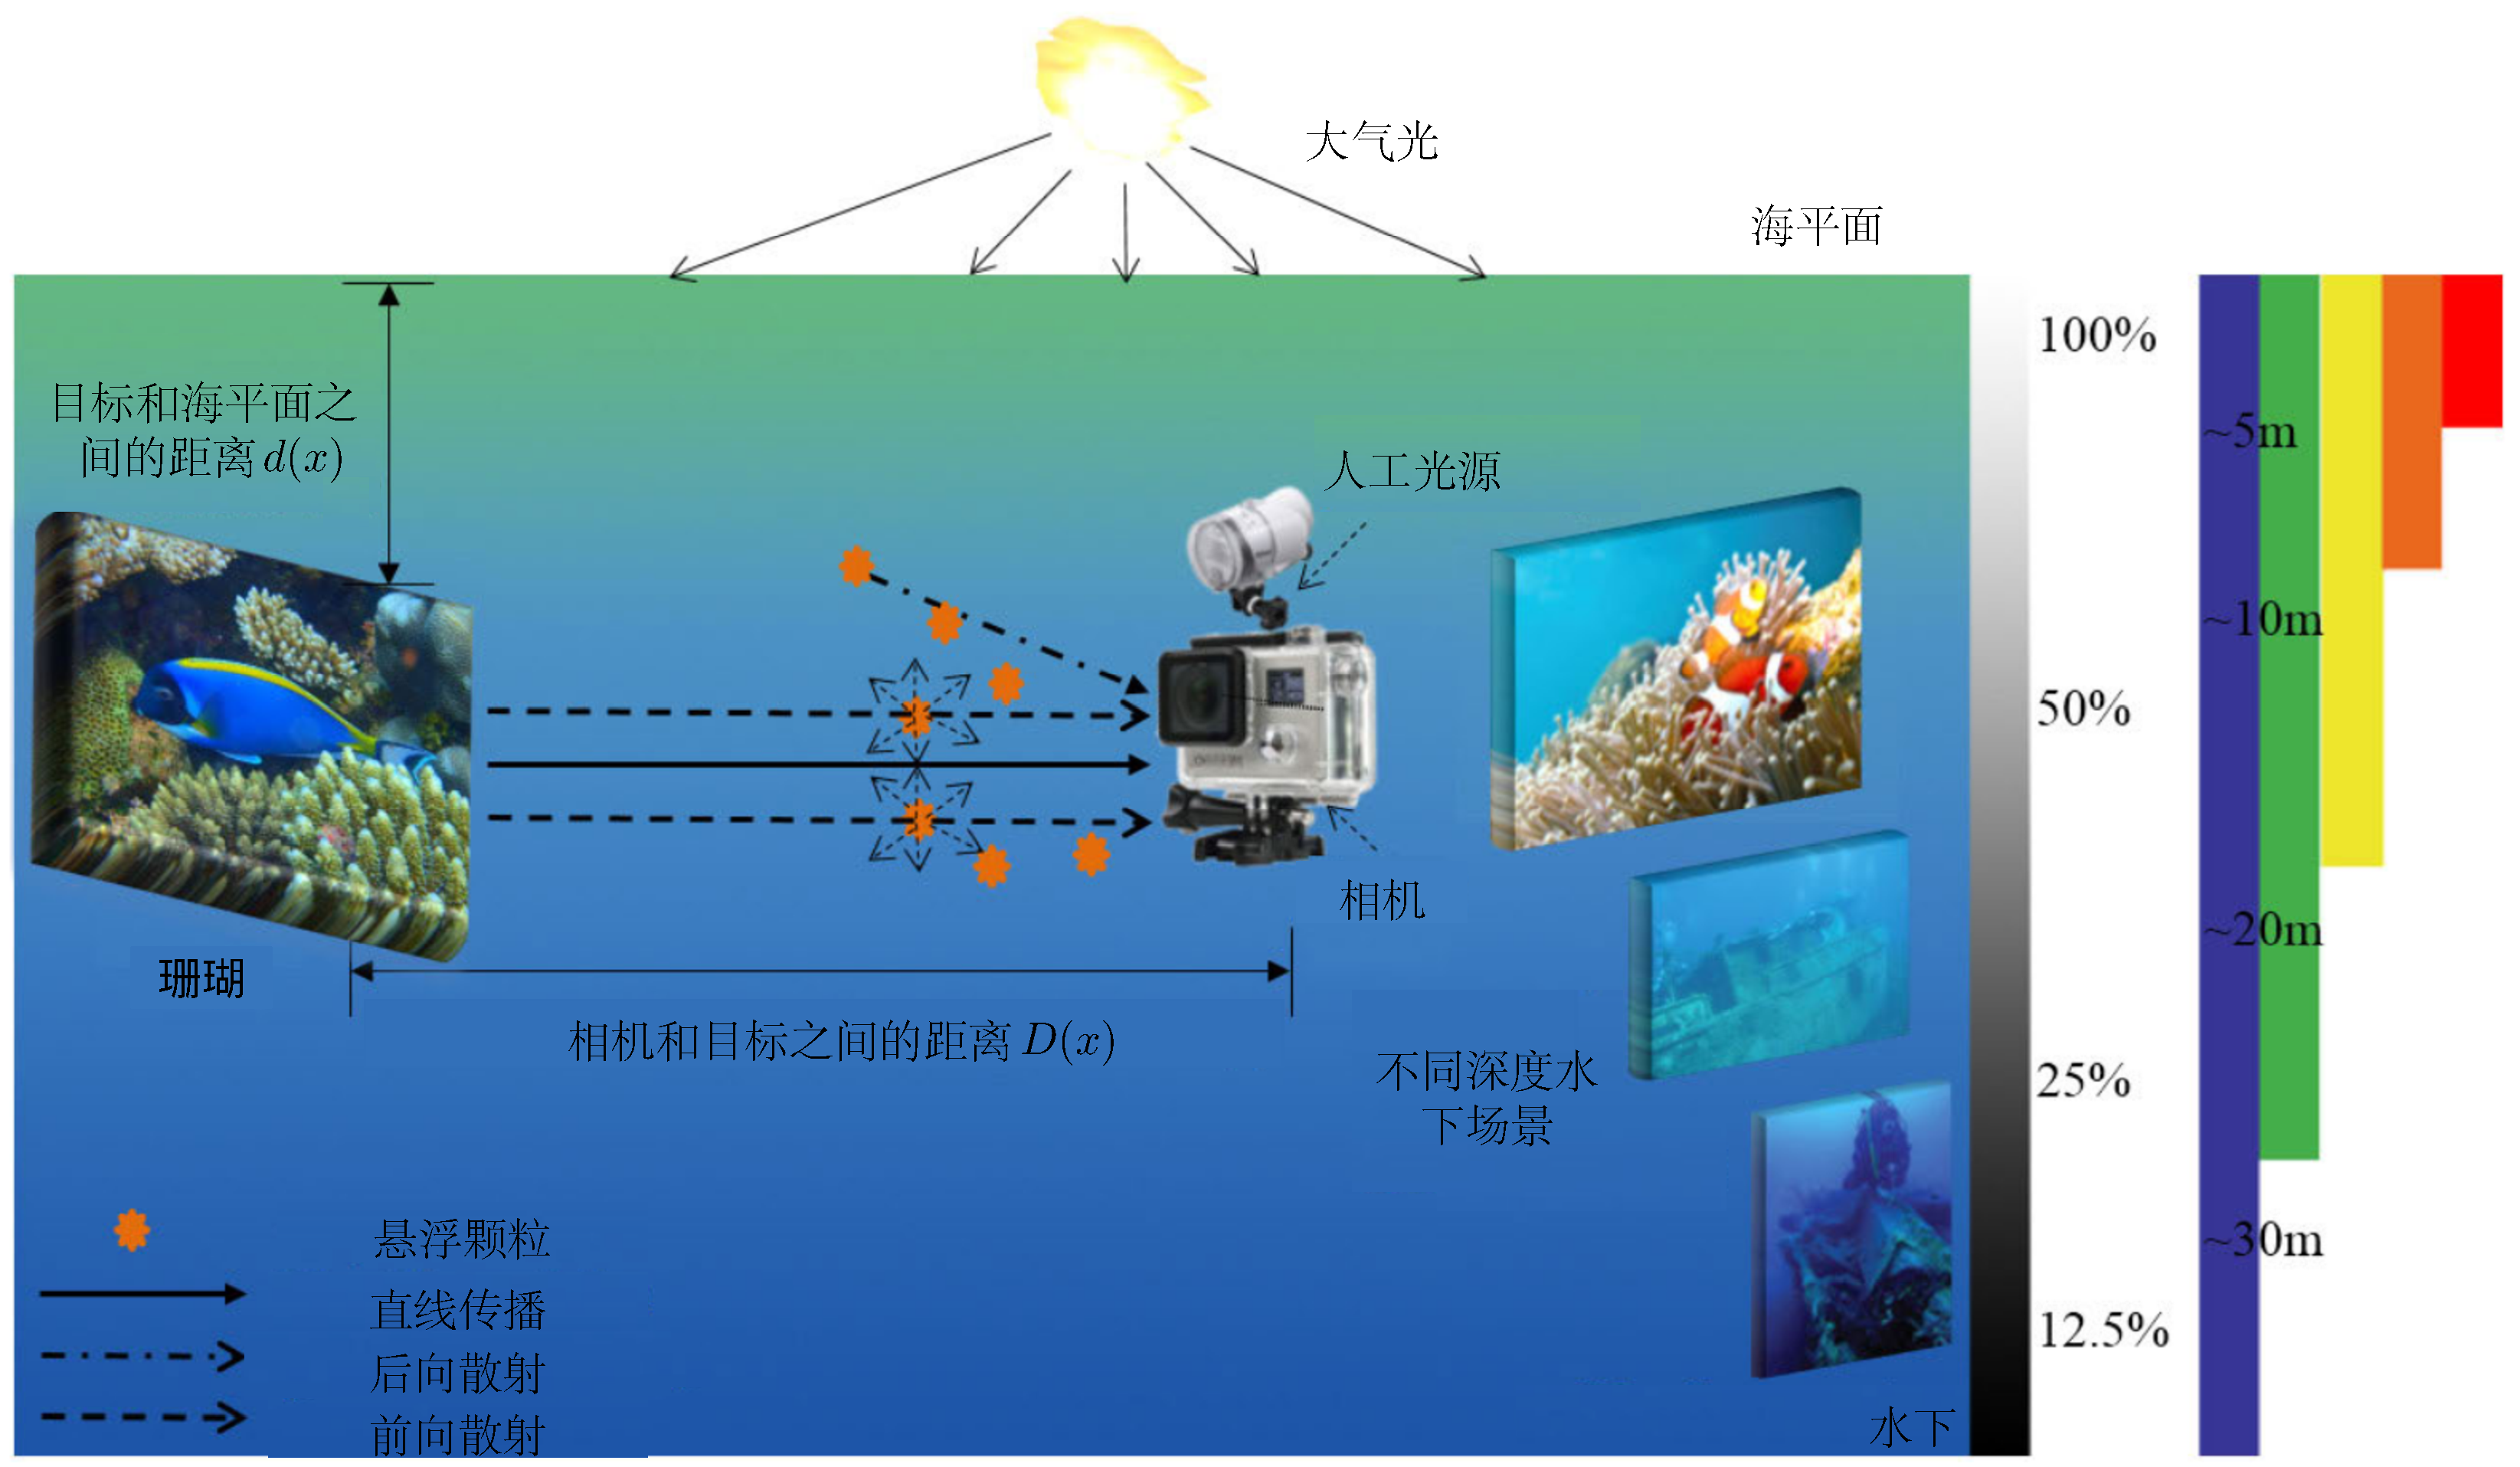
\includegraphics[width=\textwidth]{figures/水下成像.pdf}
	\caption{水下光学成像原理图。}
	\label{fig:underwater}
\end{figure*}

水下图像存在色偏的问题,图像视觉上会呈现蓝色、绿色和蓝绿色。这是由于不同颜色的光在水中的衰减特性造成的,红光波长较长,蓝色和绿色光波长较短,在水介质中光的传播过程中波长较长的光吸收速度更快,因此水下图像都是呈现蓝绿色调。

水下采集到的图像会存在对比度低,模糊的问题。吸收和散射,即悬浮在水中的颗粒吸收了传播中的大部分光,并将水下场景的反射光在到达相机前改变了光的方向,水的浑浊严重降低了图像质量。人为光线除了吸收和散射,还会出现照明不均匀以及照明不足的问题,会造成阴影。

%水下成像公式

此外,由于水下环境的成像需要耗费巨大的人力和物力资源,水下图像数据量远远小于非水下自然场景的图像数据量,配对的多模态图像结果的获取更难能可贵。缺少水下图像数据给水下视觉研究造成巨大的困难,这也是研究人员针对水下视觉进行大量工作的原因。

\section{水下图像合成研究}
\subsection{水下图像数据集}
由于真实水下场景的配对数据集数量有限,在水下视觉工作中也常用合成水下数据集进行研究。常用的真实数据集和合成水下数据集有如下几种,在我们实验中,根据实验设计将数据集组合进行使用,以达到训练目的。

RUIE~\cite{liu2019real}是共四千多的大规模真实水下数据集。针对可见度增强的性能进行评估的水下图像质量子集,包含五种质量的水下图像其中每种726张,用来测试水下图像增强效果;评估在不同照明和色偏算法的子集,包含蓝色、绿色以及蓝绿色三种色偏的水下图像每种100张;对高级计算机视觉任务如分类和检测的子集,包含对扇贝、海参和海胆三种海洋生物的标注每种100张。

UIEB~\cite{li2019underwater}是具有多样性场景、数量大以及具有高质量参考图像的成对真实场景数据集。原始图像图像共有950张,具有参考图像配对结果的890张,其余60张没有对应的参考图像。采用12种图像增强方法来进行图像增强,针对每张原始图像50个志愿者来选出令人满意的图像增强结果作为真值,令半数以上人不满意的60结果作为挑战图像没有真值。

像以上这种水下图像数据集相比较于非水下场景(空中)图像数量非常少,进行水下视觉图像研究时,研究人员会按照任务需要将空中图像进行水下环境条件模拟,合成该输入对应环境下的水下图像。

UWCNN~\cite{li2020underwater}论文中提出的从地面图像得到相应水下图像数据集。通过RGB-D NYU-v2~\cite{Silberman:ECCV12}室内数据集生成10种类型的水下图像。RGB-D NYU-v2室内共1449张图像,其中的1000张用于训练,剩下的449张用于测试,数据集提供的10类水图像也是共1449张图像。对于每张室内图像,根据生成的随机均匀全球大气光和深度(从0.5米到15米,每张图像生成5张水下图像。RGB-D NYU-v2室内数据集中的图像作为ground truth(真图),和合成的水下图像(假图)配对。

EUVP是UGAN~\cite{fabbri2018enhancing}中提出数据集的基础上更加齐全的数据集。UGAN中,ground truth是真实的相对不失真的水下图像(真图),配对的是生成的失真的水下图像(假图)。从ImageNet中选择一些不失真的水下图像,组成X域,共6143张图像,再从ImageNet中选择一些有明显水下图像特点的水下图像,组成Y域,共1817张图像。用CycleGAN实现风格迁移,即将X域中不失真的图像转成Y域中失真水下图像的风格(主要是颜色的变化)。最终用于训练的图像对是将X域中的图像都转译成失真水下图像。EUVP中,分为paired和unpaired两种。Paired文件夹中包含3个子文件夹:Underwater Dark、Underwater ImageNet和Underwater Scenes,其中Underwater Dark有5550个图像对,570张验证图像,共11670张;Underwater ImageNet有3700个图像对,1270个验证图像,共8670张图像;Underwater Scenes有2185个图像对,130个验证图像,共4500张图像。Unpaired:poor quality中有3195张,good quality中有3140张,validation中有330张,共6665张图像。

UVB 2017是一个模拟图像和视频数据集,是我们实验室在大连用ZED和Kinect摄像机进行拍摄的。用不同\ce{Al(OH)3}的浓度来模拟不同水质类型的衰减系数,摄像机收集了目标物在不同水质下的各种结果。已整理好的数据文件包括衰减为0即无水环境下的采集结果、衰减为1.2、1.58至衰减系数为3的多种结果。数据集在浑浊程度上随着衰减系数增加有视觉可见的从清晰到浑浊的变化过程。

\subsection{水下图像评价指标}
UCIQE~\cite{yang2015underwater}和UIQM~\cite{panetta2015human}是无参考/无真值评价水下图像质量的常用指标,是评价水下图像质量的关键指标。

UCIQM是色彩浓度,饱和度和对比度为测量分量的线性组合,可以定量的评价水下增强结果的色偏、模糊和对比度情况。属于无参考/无真值的图像质量评价指标,首先将水下图像从RGB颜色空间转换到CIELab颜色空间,这样更符合人类视觉感知,然后计算个测量分量,具体计算如式~\ref{equ:uciqe}所示。

\begin{equation}
\label{equ:uciqe}
UCIQE = c_1 \times \sigma_c + c_2 \times con_l + c_3 \times \mu_s
\end{equation}

其中,$ \sigma_c$为色度的标准方差,$con_l$为亮度的对比度,$\mu_s$是饱和度的平均值,$c_1$,$c_2$和$c_3$分别为线性组合的权重值。

UIQM针对水下图像的退化机理和成像特点,采用色彩测量UICM,清晰度测量UISM和对比度测量UIConM作为评价水下图像质量的依据。UIQM属于无参考/无真值的图像评价指标,通过测量分量的线性组合来表征图像的视觉质量,如式~\ref{equ:uiqm}所示。

\begin{equation}
\label{equ:uiqm}
UIQM = c_1 \times UICM + c_2 \times UISM + c_3 \times UIConM
\end{equation}

其中,$c_1$,$c_2$和$c_3$分别为线性组合的权重值,权重值的设定需要视具体任务而定,评价水下图像的颜色偏差修正结果时,需设定色度测量分量UICM更大的权重因子;当评价对比度和清晰度时,需要设定清晰度测量分量UISM和对比度测量分量UIConM更大的权重因子。

尽管,两种无参考的指标一定程度上给出定量的图像评价分数,但缺点也很明显。首先,水下图像质量不佳的视觉类型较多,仅参考几个测量分量的线性组合对于图像评价是片面的,缺少客观性和准确性;其次,测量分量权重的设置具有主观性,难以公正的评价水下图像质量;最后,评价结果域视觉效果不一致,会出现指标指示评价较好但视觉上没有直观的展现图像的优越性。


\subsection{经典水下图像合成方法}
目前现有的水下图像合成,目前有两种基本思路。一种是基于水下光学物理模型将额外的水下信息,像深度图和传输图等信息加到输入图像上,使输入图像合成具有对应深度或者浑浊度的水下结果。另一种是基于无监督的图像转译模型CycleGAN,两个域分别是空中图像域和水下图像域,通过循环一致性限制,使得空中域中的图像学习到水下域方向上图像的转译。

基于水下光学物理模型的水下图像合成方法主要如下:

WaterGAN~\cite{li2017watergan}提出无监督的水下图像色彩矫正模型。RGB-D的地面图像数据集和水下图像样本集作为输入使用WaterGAN合成与RGB-D对齐的相应水下结果,用生成的水下结果和地面结果作为配对数据训练图像复原模,测试使用真实的水下图像,输出矫正后的图像和相对深度图。

Underwater-GAN~\cite{yu2018underwater}基于水下成像模型,使用浑浊度模拟器来模拟衰减的水下图像。生成数据集一般需要收集包括真实图像和对应深度图,在Underwater-GAN中设置相应的散射系数作为深度信息,根据模型计算出散射系数来合成相对应的水下图像。

UWGAN~\cite{wang2019uwgan}将彩色RGB图像及其深度图作为输入,然后通过生成对抗性训练学习参数,从而基于水下光学成像模型合成不同类型的水下真实图像。提出用于水下图像恢复和增强的U-net体系结构,比较了U-net中不同损失函数的影响,在此基础上提出了最适合水下图像恢复的损失函数。


UIE-DAL~\cite{uplavikar2019all}提出水下增强模型,问题是水类型的多样性使得难以用一个模型来完美实现全部水类型的增强,该工作提出一个Encoder-Decoder卷积网络结构,将不同水类型视为不同域消除相应干扰来学习图像的内容特征。其中合成图像数据集同UWCNN一样将NYU v2深度数据集合成10种Jerlov风格水样作为训练数据,UIEB作为测试数据。Encoder将图像编码到潜在空间时,还进行了水样类型判别,帮助Decoder重建出不带水样类型的增强图像结果。

UWCNN~\cite{li2020underwater}是一种基于卷积神经网络的经典图像增强模型。在NYU v2~\cite{Silberman:ECCV12}深度数据集上,将海洋光学成像原理利用深度图应用于合成十种不同类型的水下图像,针对每种水下矮图像类型分别训练多个UWCNN模型,能够模拟各种退化的水下图像以进行水下数据增强。训练集使用NYU v2数据集合成配对的十种类型水样,测试集选择网络上的水下真实图像测试训练好的每种水样类型的效果。

基于无监督图像转译模型CycleGAN的水下图像合成方法主要如下:

UGAN~\cite{fabbri2018enhancing}使用CycleGAN来生成水下图像,从而为进行颜色矫正提供数据。在整个过程中,需要在水下和陆地两个单独的域中拍摄物体图像。使用生成对抗网络作为生成模型,构造将水下图像的真实外观估计变成成对图像转译问题,使用来自两个域的图像作为输入和真值。使用ImageNet的子集来训练和评估网络性能。UGAN-P是在UGAN基础上加入梯度差异损失,直接惩罚生成器中图像梯度预测的差异来增强预测。

MLFcGAN~\cite{liu2019mlfcgan}提出一种基于条件生成对抗网络的深度多尺度特征融合网络,主要用于进行颜色校正问题,数据集使用UGAN中提出的,并且从网上找了多张真实场景的水下图像来评价模型的泛化能力。

总而言之,在上述提到的水下图像合成方法中,主要分成两种类型的合成。一种是利于水下光学成像原理,利用深度图或者传输图等水下信息作为水下条件将空中图像模拟合成相对应的水下场景图像,如WaterGAN,UWCNN,UWGAN,Underwater-GAN和UIE-DAL。依赖这种方法始终无法摆脱物理模型的控制,需要深度图/传输图等信息作为指引;且生成水下图像类型固定,若要生成多样化结果需要训练多个模型依次对应。另一种是利用无监督一对一映射的图像转译方法CycleGAN,使用不成对的数据即可进行水下图像合成,如UGAN和MLFcGAN。

\section{水下图像多模态合成研究}
针对水下图像多模态合成任务,我们旨在用一个模型不需额外信息一次实现多种模态样式的合成。在水下视觉任务中,水下图像合成的常用方法中,用无监督图像转译模型CycleGAN只能实现一对一映射,合成结果是单模态,缺乏多样性。使用光学成像原理图像合成方法,经过多次执行可以获得多模态样式的结果,但是需要重复执行合成流程,且需要补充相对应的深度图或者传输图等水下条件信息作为模态样式的引导,若数据集中不存在这种水下条件信息,则无法在该数据集上进行使用,因此深受数据限制,泛化能力有限。

我们希望通过一个网络模型,仅给定不配对的水下图像数据进行训练,就可以将给定图像合成多种模态样式的水下结果。为了解决这个问题,可以借鉴我们研究的基于生成对抗网络的无监督图像域转译的方法,根据水下图像的特点,重新设计相应有效的转译模型,从而实现将给定图像到多模态图像的合成。这样就可以实现从输入到输出一对多的映射及图像合成,从而避免需要额外的信息而对数据有较高的要求并限制住模型的泛化能力。

因此,基于以上图像转译和水下图像合成内容的研究,针对水下图像多模态合成问题,有两种设计思路,如下分析并设想了两种水下图像多模态合成模型。

第一种,将空中图像和水下多模态图像视为两个域,将该问题转化成跨域的多模态转译问题。受到图像转译中UNIT,MUNIT,DRIT等经典分解表示学习工作的启发,可以设计一种针对水下跨域多模态转译模型,将图像拆分成内容和样式两部分内容,目的是实现在多模态转译过程中让多个模态之间内容保持不变,仅通过目标域的随机采样或者参考进行引导,模态达到目标域给定水样式或者模糊程度上的变化。

另一种,将空中图像和水下图像的多种水类型都视为多个域,将多个类型风格之间的转译转化成多域的转译问题。收到UIE-DAL启发,也可以通过编码进行多种风格域之间的控制,通过一个网络将编码影响带入合成结果,类似多域图像转译模型StarGAN一样,用编码进行域转译控制,目的是转译合成图像时多个模态之间内容应相同,仅不同编码控制实现的目标风格样式不同,编码可以是水颜色、模糊程度等水下环境条件。


\section{本章小结}
本章主要对水下图像进行研究,并提出相对应的设计思路,分析和设计研究水下图像多模态转译提供理论基础和数据支撑。

第一小节,介绍并分析了水下图像的成像原理、特点和存在的问题。通过对水下图像的特点进行详细了解和分析,为后续完成水下图像合成任务打下理论基础。

第二小节,对水下合成任务进行研究。简要介绍了水下任务中常用数据、水下图像评价指标和经典的水下图像合成方法。针对这些经典水下图像合成任务中的方法进行总结,分析其各种利弊,为后续设计多模态图像合成任务开拓思路。

第三小节,水下图像多模态合成研究。阐述了我们水下图像多模态合成任务的目的和独特性,针对水下图像多模态合成任务,设想出合理可行的设计思路。后续将对提出的思路进行具体网络设计、实验并给出实验结果,对每种思路在视觉上和指标上给出直观的结果展示。